
\begin{figure}
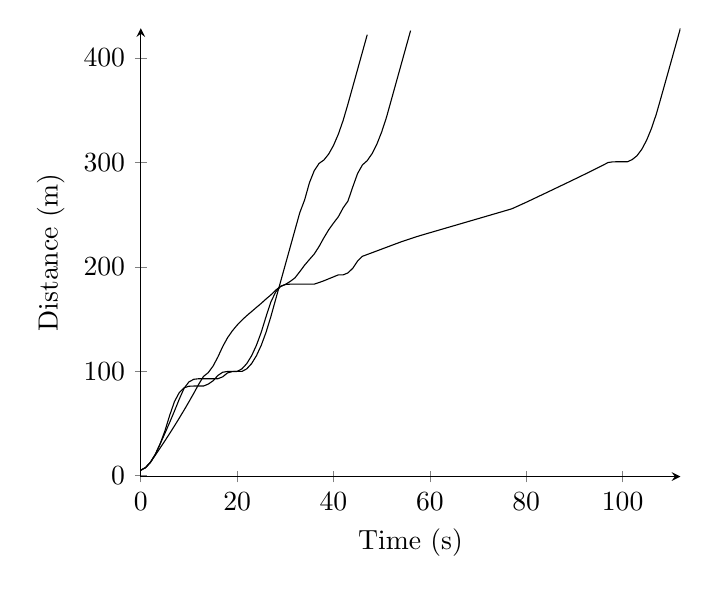
\begin{tikzpicture}
\begin{axis}[
legend style={anchor=west},
axis x line=bottom,
axis y line=left,
ymin=-1,
xlabel=Time (s),
ylabel=Distance (m),
]
\addplot[] coordinates {
(0, 5.1)
(1, 7.6)
(2, 12.6)
(3, 20.1)
(4, 30.0491286981)
(5, 40.2916206764)
(6, 50.8706103169)
(7, 61.8381932978)
(8, 73.2578967178)
(9, 83.6753638918)
(10, 89.6971616909)
(11, 92.1978704104)
(12, 92.6981430277)
(13, 92.7189629629)
(14, 92.7189629629)
(15, 92.7189629629)
(16, 92.7189629629)
(17, 94.550969567)
(18, 98.28216385)
(19, 99.5796999959)
(20, 99.71839693)
(21, 99.71839693)
(22, 102.21839693)
(23, 107.21839693)
(24, 114.71839693)
(25, 124.71839693)
(26, 137.21839693)
(27, 152.21839693)
(28, 168.81839693)
(29, 185.41839693)
(30, 202.01839693)
(31, 218.61839693)
(32, 235.21839693)
(33, 251.81839693)
(34, 263.95839693)
(35, 280.459491055)
(36, 292.017569177)
(37, 299.040209842)
(38, 302.276956125)
(39, 308.013702408)
(40, 316.250448691)
(41, 326.987194974)
(42, 340.223941258)
(43, 355.960687541)
(44, 372.560687541)
(45, 389.160687541)
(46, 405.760687541)
(47, 422.360687541)
};
\addplot[] coordinates {
(0, 5.1)
(1, 7.6)
(2, 12.6)
(3, 20.1)
(4, 30.1)
(5, 42.6)
(6, 57.6)
(7, 70.9171823702)
(8, 79.5329710754)
(9, 84.0321050879)
(10, 85.5315855274)
(11, 85.7161179745)
(12, 85.7161179745)
(13, 85.7161179745)
(14, 87.5597713287)
(15, 90.7285776244)
(16, 95.8361082111)
(17, 98.9249310978)
(18, 99.6733254866)
(19, 99.7198198561)
(20, 99.7198198561)
(21, 102.219819856)
(22, 107.219819856)
(23, 114.719819856)
(24, 124.719819856)
(25, 137.219819856)
(26, 152.219819856)
(27, 166.3376613)
(28, 175.829459476)
(29, 181.065398495)
(30, 183.028755665)
(31, 183.341819214)
(32, 183.341819214)
(33, 183.341819214)
(34, 183.341819214)
(35, 183.341819214)
(36, 183.341819214)
(37, 184.887808669)
(38, 186.584209661)
(39, 188.465889958)
(40, 190.347620091)
(41, 192.229402364)
(42, 192.229402364)
(43, 194.143684127)
(44, 198.55796589)
(45, 205.472247653)
(46, 210.034304489)
(47, 211.761440631)
(48, 213.488669791)
(49, 215.215996834)
(50, 216.943426971)
(51, 218.670965793)
(52, 220.398619301)
(53, 222.126393946)
(54, 223.829310002)
(55, 225.402948026)
(56, 226.948685868)
(57, 228.488777691)
(58, 229.903540012)
(59, 231.267966745)
(60, 232.618285231)
(61, 233.965284506)
(62, 235.311685301)
(63, 236.658129093)
(64, 238.004769354)
(65, 239.35165156)
(66, 240.698798992)
(67, 242.046231536)
(68, 243.393969821)
(69, 244.742036264)
(70, 246.090286978)
(71, 247.438857552)
(72, 248.787918313)
(73, 250.137454786)
(74, 251.487481864)
(75, 252.838034476)
(76, 254.189157423)
(77, 255.540902512)
(78, 257.626825021)
(79, 259.713545788)
(80, 261.833167799)
(81, 264.001831561)
(82, 266.19145116)
(83, 268.383579034)
(84, 270.578579423)
(85, 272.776891674)
(86, 274.979050971)
(87, 277.185716452)
(88, 279.397710052)
(89, 281.616071273)
(90, 283.842136276)
(91, 286.077655262)
(92, 288.324972475)
(93, 290.587313198)
(94, 292.869263858)
(95, 295.177625172)
(96, 297.523052471)
(97, 299.92356785)
(98, 300.574405459)
(99, 300.609601363)
(100, 300.609601363)
(101, 300.609601363)
(102, 302.733716007)
(103, 306.45561952)
(104, 312.677523033)
(105, 321.399426546)
(106, 332.621330059)
(107, 346.343233572)
(108, 362.565137085)
(109, 379.000261557)
(110, 395.479436729)
(111, 411.990838604)
(112, 428.590838604)
};
\addplot[] coordinates {
(0, 5.1)
(1, 7.6)
(2, 12.6)
(3, 19.3264940681)
(4, 26.1762904273)
(5, 33.1610343725)
(6, 40.2938980128)
(7, 47.5898407731)
(8, 55.0659254002)
(9, 62.7417038242)
(10, 70.6396916417)
(11, 78.785955987)
(12, 87.21084981)
(13, 94.85305646)
(14, 98.5691936801)
(15, 104.7853309)
(16, 113.50146812)
(17, 123.483763642)
(18, 131.938527248)
(19, 138.564939342)
(20, 144.115592663)
(21, 148.914103507)
(22, 153.181169172)
(23, 157.075753468)
(24, 161.063745727)
(25, 164.939227863)
(26, 169.140266017)
(27, 173.051487927)
(28, 177.540104463)
(29, 181.294756477)
(30, 183.03969826)
(31, 185.92404029)
(32, 189.363929935)
(33, 195.303819581)
(34, 201.521493856)
(35, 206.949786575)
(36, 212.232968136)
(37, 219.400035684)
(38, 227.742713223)
(39, 235.413221016)
(40, 241.86378665)
(41, 247.895066493)
(42, 256.426346337)
(43, 262.997626181)
(44, 276.528906025)
(45, 289.382370632)
(46, 297.567276427)
(47, 301.715807497)
(48, 308.364338567)
(49, 317.512869636)
(50, 329.161400706)
(51, 343.309931776)
(52, 359.909931776)
(53, 376.509931776)
(54, 393.109931776)
(55, 409.709931776)
(56, 426.309931776)
};

\end{axis}
\end{tikzpicture}
\label{tik:100:14_V, 15_N, 17_S, 17_S.-60, 19_V}
\caption{100 percent diving with GSC on route $14_V, 15_N, 17_S, 17_S.-60, 19_V$}
\end{figure}
